
\chapter{Functions}

This chapter covers the following ideas. 

% A list of objectives for the chapter
%\begin{enumerate}
%\item ...
%\end{enumerate}


\begin{enumerate}
\item Be able to describe cylinders and quadric surfaces in space.
\item Describe uses for function with varying input and output
  dimensions.  Be able to draw appropriate representations when the
  input and output dimensions are 3 or less. Recognize by name and
  graph the different types of functions, in particular parametric
  equations, space curves, functions of several variables, vector
  fields, transformations, and parametric surfaces.
\item Find derivatives of space curves, and use the derivative to find
  tangent lines to space curves.
\end{enumerate}


%%% Local Variables: 
%%% mode: latex
%%% TeX-master: "../multivariable-calculus"
%%% End: 
%$



\section{Cylinders and Quadric Surfaces}

\subsection{Cylinders}
A right circular cylinder is formed by taking a circle in a plane
(hence the word ``circular''), and then extending through each point
of the circle a straight line with direction vector orthogonal (hence
the word ``right'') to the plane.  In general, a cylinder is any
surface which is created by extending through each point of a curve a
straight line in a fixed direction.  The curve through which the lines
are drawn is called a generating curve for the cylinder. The
intersection of a cylinder with a coordinate plane is called a
\emph{cross-section} or a \emph{trace}. Some examples of cylinders are
below, where the generating curve is in bold.
\newcommand{\mywidth}{1.0in}
\begin{center}
\begin{tabular}{cccc}
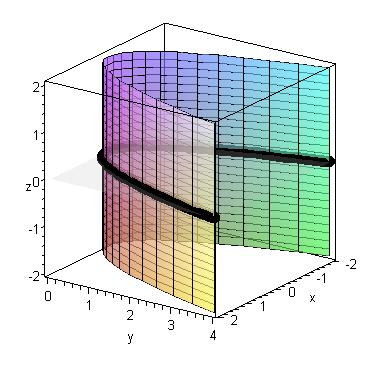
\includegraphics[width=\mywidth]{functions/cylinder-1}&
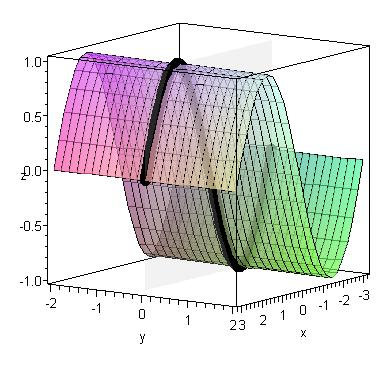
\includegraphics[width=\mywidth]{functions/cylinder-2}&
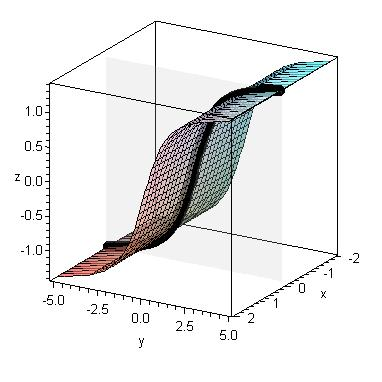
\includegraphics[width=\mywidth]{functions/cylinder-3}&
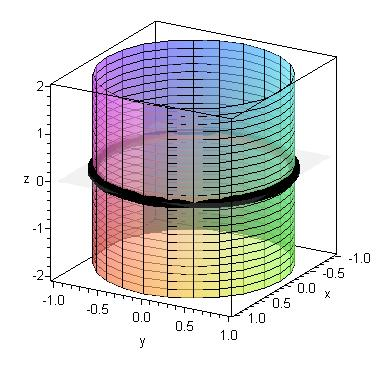
\includegraphics[width=\mywidth]{functions/cylinder-4}
\\
$y=x^2$ &
$z=\sin(x)$ &
$y=\tan(z)$ &
$x^2+y^2=1$
\end{tabular}
\end{center}

\subsection{Quadric Surfaces}
A quadric surface is a generalization of conic sections to three
dimensions.  In general, it is the graph in 3D of any expression
involving at most second degree terms in $x$, $y$, and/or $z$. To
graph a quadric surface, hold one variable constant and then graph the
resulting conic section in the plane which represents the variable you
held constant. Repeat this for a few different variables and constants
until you can piece together the surface.  An example of this process
for $\frac{x^2}{4}+\frac{y^2}{9}-z^2 =1$ is illustrated below, as well
as some typical quadric surfaces.  \renewcommand{\mywidth}{.9in}
\begin{center}
\begin{tabular}{cccc}
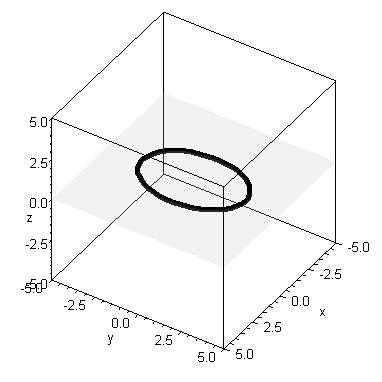
\includegraphics[width=\mywidth]{functions/quadric-1}&
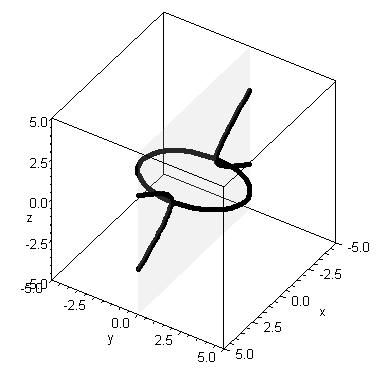
\includegraphics[width=\mywidth]{functions/quadric-2}&
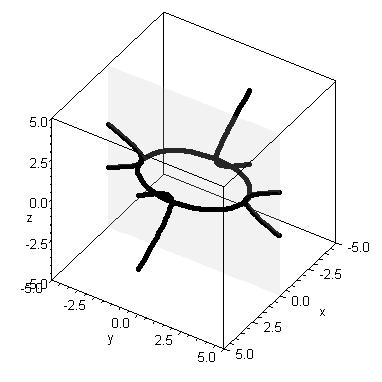
\includegraphics[width=\mywidth]{functions/quadric-3}&
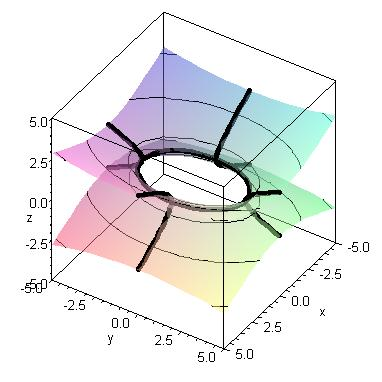
\includegraphics[width=\mywidth]{functions/quadric-4}
\\
Let $z=0$ &
Let $y=0$ &
Let $x=0$ &
$\frac{x^2}{4}+\frac{y^2}{9}-z^2 =1$\\
&&&Hyperboloid of one sheet
\\
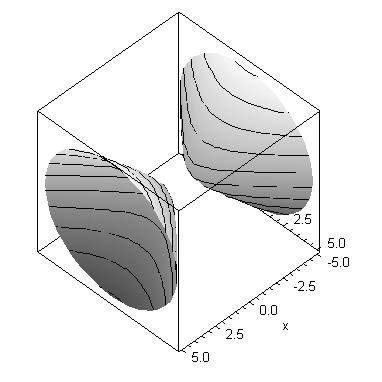
\includegraphics[width=\mywidth]{functions/quadric-5}&
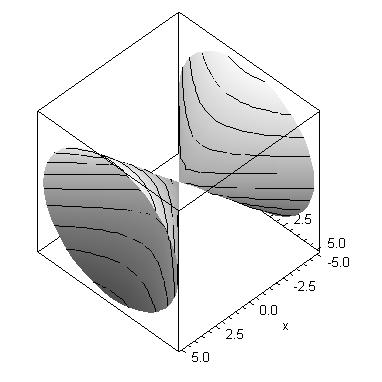
\includegraphics[width=\mywidth]{functions/quadric-6}&
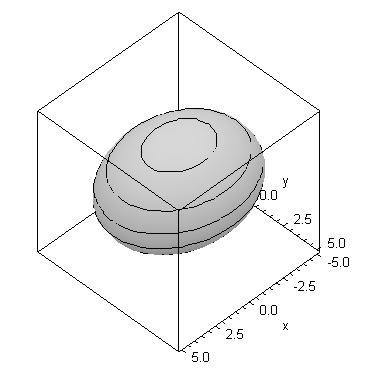
\includegraphics[width=\mywidth]{functions/quadric-7}&
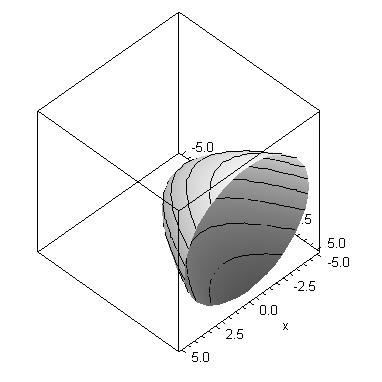
\includegraphics[width=\mywidth]{functions/quadric-8}
\\
$x^2-y^2-z^2=1$ &
$-x^2+y^2+z^2=0$ &
$\frac{x^2}{25}+\frac{y^2}{16}+\frac{z^2}{9}=1$ &
$x^2-4y+z^2=1$
\\
Hyperboloid of 2 sheets&
Cone &
Ellipsoid &
Paraboloid
\end{tabular}
\end{center}






\section{Function terminology}
A function is a set of instructions (a relation) involving two sets
(called the \emph{domain} and \emph{codomain}).  A function assigns to
each element of the domain $D$ at most one element in the codomain
$R$. It is customary to write {$f\colon D\to R$} when we want to
specify the domain and codomain.  Not all elements of $R$ may be
assigned; the set of elements in $R$ that are assigned is called the
\emph{range} of the function.
\note{drawing of the domain, range, and codomain circles, with the function arrow going between}

\begin{example}
  If the function $f(x)=x^2$, then the domain and codomain are typically
  $\RR$ (i.e., $f\colon \RR \to \RR$), and the range is the set of nonnegative numbers.
\end{example}

In this class, we will study what happens when the domain and codomain
are subsets of {${\RR}^n$} ($\RR^n$ is the set of all $n$-dimensional
real points, and is often called ``Euclidean {$n$}-space''). In
particular we will study functions of the form $f\colon {\RR}^n\to
{\RR}^m$.

\section{Functions: $\RR^n\to \RR$}
\subsection{Functions of one variable: $f\colon \RR^1\to  \RR^1$}
In the first year of calculus, the domain and codomain are always
subsets of the real numbers {$\RR$}.  A typical example is $f(x)=x^2$.
Many ideas like derivatives, integrals, etc., from first semester
calculus generalize to all dimensions, but some do not.

\subsection{Functions of several variables:  $f\colon \RR^2\to \RR$, $f\colon \RR^3\to \RR$, $f\colon \RR^n\to \RR$} 

With functions of this type, the output dimension is always 1, while
the input dimension may be as large as needed. This type of function
is used to measure a quantity at each point in the plane ($f\colon {\RR}^2\to
{\RR}$), at each point in space ($f\colon {\RR}^3\to {\RR}$), or for every
combination of $n$ inputs ($f\colon {\RR}^n\to {\RR}$). The temperature at
each point in the plane would be modeled by such a function of the
form $T(x,y)$. The wind speed at each point in space could be modeled
by a function of the form $f(x,y,z)$.

To graph functions of the form {$f\colon {\RR}^2\to {\RR}$}, we typically
write $z=f(x,y)$ and then plot the function in $xyz$ coordinates.
Every pair $(x,y)$ corresponds to exactly one point $(x,y,f(x,y))$ in
space.  Functions of this form still pass the ``vertical line test''
(where ``vertical line'' means a line parallel to the $z$-axis).  We
get 2D traces (vertical cross sections) of the function by replacing
$x$ or $y$ with a constant and creating a 2D graph of the resulting
function.  A level curve is a graph in the plane of the equation
$c=f(x,y)$ for some constant $c$ (essentially a level curve is a
horizontal cross section drawn in the $xy$-plane). Plotting several
level curves creates a \emph{contour plot} of the function.  A few
graphs and corresponding contour plots follow.


\renewcommand{\mywidth}{1.1in}
\begin{center}
\begin{tabular}{cccc}
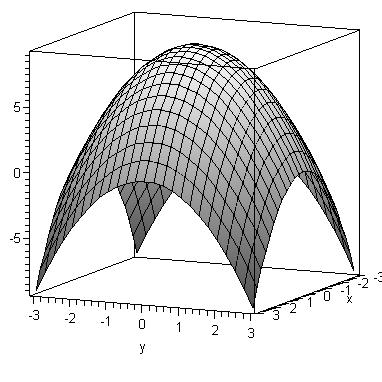
\includegraphics[width=\mywidth]{functions/functionseveral-1}&
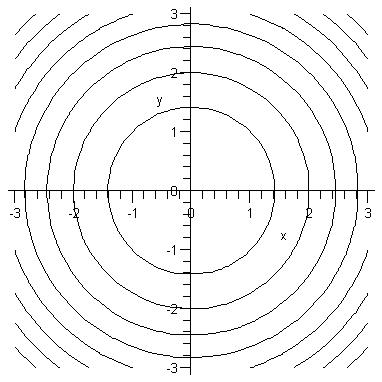
\includegraphics[width=\mywidth]{functions/functionseveral-2}&
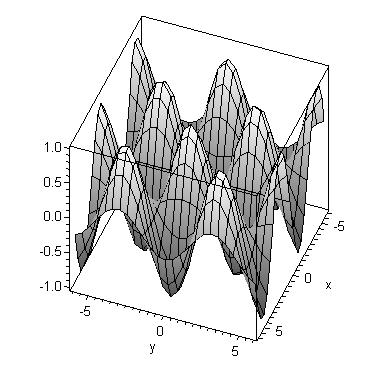
\includegraphics[width=\mywidth]{functions/functionseveral-3}&
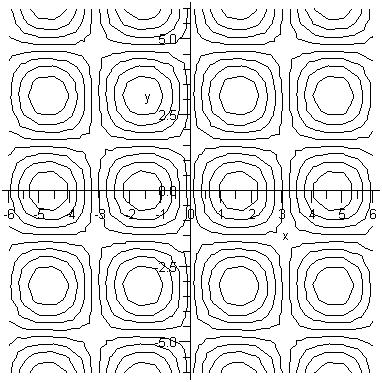
\includegraphics[width=\mywidth]{functions/functionseveral-4}
\\
$f(x,y)=9-x^2-y^2$&
level curves of $f$ &
$g(x,y) = \sin x \cos y$ &
level curves of $g$\end{tabular}
\end{center}

Functions with three inputs {$f\colon {\RR}^3\to {\RR}$} would require 4
dimensions to graph.  Rather than graph functions in 4D, we instead
look at level surfaces. For the function $w=f(x,y,z)$, we pick a
constant $w=c$ and graph the surface $c=f(x,y,z)$.  The level surface
$w=1$ for the function $f(x,y,z)=x^2+y^2+z^2$ is a sphere of radius 1
(given by graphing $x^2+y^2+z^2=1$).  Quadric surfaces will show up
often when you graph level surfaces of functions with three inputs.


\section{Parametric Functions}

\subsection{Parametric curves: {$\vec r\colon \RR\to \RR^2$}}
Parametric curves often represent motion in the plane.  We can write
these functions by giving the equations for each coordinate
separately, or we can write all of the equations as a vector, where
each coordinate of the vector is a function of one variable.  Because
these output of these functions is a vector, we call these functions
\emph{vector-valued functions}, and often emphasize this by writing
them with a vector symbol over the name.


\begin{example}
  The parametric curve $x=2\cos t$, $y=3\sin t$ traces out an ellipse.
  We can also write this in vector form as $\vec r(t) = \langle2\cos
  t, 3\sin t\rangle$.
\end{example}

\subsection{Spacecurves: {$\vec r\colon \RR\to \RR^3$}}
Space curves generalize parametric curves, but the outputs are
three-dimensional points, so these are curves in space.  The notation
{$\vec r\colon \RR \to \RR^3$} suggests that we are graphing a
one-dimensional object in three dimensions. The graph of a space curve
looks like a bent wire in space, or as a path of motion traced out in
space.  For each time $t$, the position vector $\vec r(t)$ gives the
position of a particle whose motion is described by the space curve.
Again, since the output is a vector, a space curve is a vector-valued
function.  Just like a 2D parametric plot, a space curve can graphed
by picking values for $t$ and plotting the corresponding points $\vec
r(t)$.

The derivative of a space curve is found by differentiating each
component of the space curve, which follows immediately by looking at
the limit $\ds\frac{d\vec r}{dt}=\lim_{h\to 0}\frac{\vec r(t+h)-\vec
  r(t)}{h}$. An equation of the tangent line to a space curve at $t=c$
has direction vector equal to $\dfrac{d\vec r}{dt}$ (evaluated at
$t=c$) and passes through the point $\vec r(c)$, and so has an equation of
$\vec l(u) = \vec r^\prime(c)u+\vec r(c)$. If a space curve is used to
describe motion, then velocity is $\vec v(t) = \dfrac{d\vec r}{dt}$,
speed is the magnitude of velocity $|\vec v|$, and acceleration is
$\vec a(t) = \dfrac{d\vec v}{dt}$, just as was taught in first-semester
calculus for single-variable functions.


\renewcommand{\mywidth}{0.9in}
\begin{wrapfigure}[6]{r}{0pt}
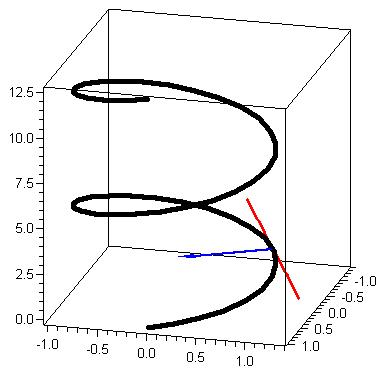
\includegraphics[width=\mywidth]{functions/spacecurve-1}
\end{wrapfigure}
\examplebegin
The space curve {$\vec r(t)=\langle\cos(t),\sin(t),t\rangle$} is a
helix which wraps around the $z$-axis.  Its graph is shown on the
right, where $0\leq t\leq 4\pi$, as well as the tangent line and acceleration
vector. The velocity and acceleration at any time $t$ are $\vec v(t) =
\langle-\sin(t),\cos(t),1\rangle$ and $\vec a(t) =
\langle-\cos(t),-\sin(t),0\rangle$. When $t=2\pi/3$, we have $\vec
r(2\pi/3) = \langle1/2,\sqrt{3}/2,2\pi/3\rangle$, $\vec v(2\pi/3) =
\langle-\sqrt{3}/2,-1/2,1\rangle$, and $\vec a(2\pi/3) =
\langle1/2,-\sqrt{3}/2,0\rangle$. An equation of the tangent line is
$\vec l(t) = \vec v(2\pi/3)t+ \vec r(2\pi/3)=
\langle-\sqrt{3}/2,-1/2,1\rangle t+\langle1/2,\sqrt{3}/2,2\pi/3\rangle$.
\exampleend


\subsection{Parametric Surfaces: {$\vec f\colon {\RR}^2\to {\RR}^3$} }

Just as parametric and space curves describe one-dimensional objects, we use parametric surfaces to describe two-dimensional objects in 3D.  Notice that we are mapping two dimensions into three, so think of a parametric surface as a set of instructions of how to place the 2D plane in space (where you can twist the plane and stretch it based on the set of instructions).  If you hold one variable constant, then the graph of the resulting function is a space curve. To graph a parametric surface, hold one variable constant and draw the resulting space curve.  Do this for a few values of each variable, and you will have created a net of overlapping space curves from which you can piece together the surface.  

Any surface of the form $z=f(x,y)$ can be made a parametric surface by
writing $\vec r(x,y)=\langle x,y,f(x,y)\rangle$, which just says for
each $(x,y)$ to plot the point $(x,y,f(x,y))$. We often use $u$ and
$v$ as variables for a parametric surface if those variables do not
represent some other standard quantity.

\renewcommand{\mywidth}{1.4in}
\begin{center}
\begin{tabular}{cccc}
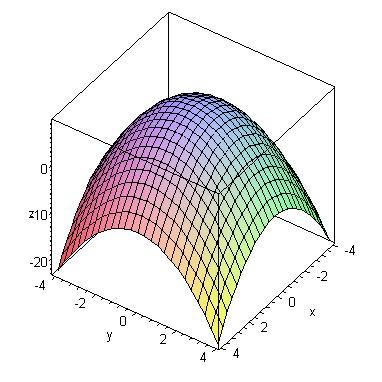
\includegraphics[width=\mywidth]{functions/parasurface-1}&
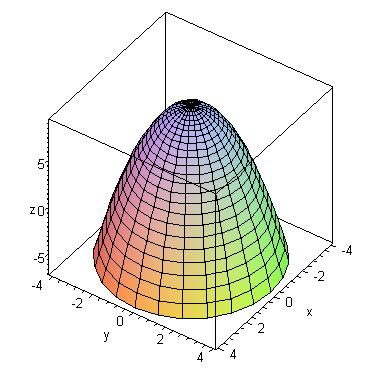
\includegraphics[width=\mywidth]{functions/parasurface-2}&
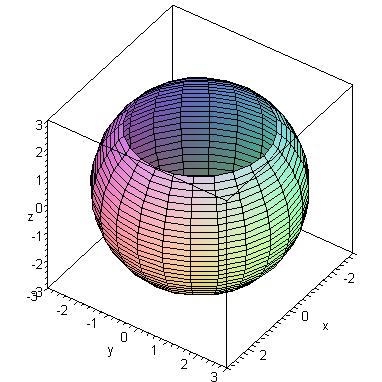
\includegraphics[width=\mywidth]{functions/parasurface-3}&
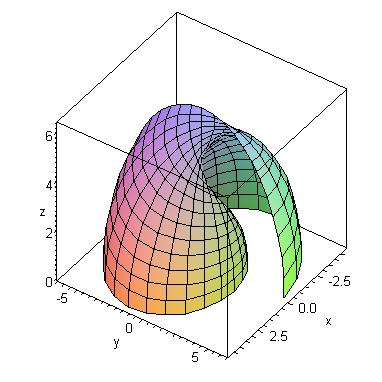
\includegraphics[width=\mywidth]{functions/parasurface-4}
\end{tabular}
\end{center}
The functions are, from left to right, 

$\vec r(x,y) = \langle x,y,9-x^2-y^2\rangle$ for $-4\leq x\leq 4,-4\leq y\leq 4$

$\vec r(u,v)=\langle u\cos v,u\sin v ,9-u^2\rangle$ for $0\leq u\leq 3,0\leq v\leq 2\pi$ (cylindrical coordinates) 

$\vec r(\theta,\phi)=\langle3\cos\theta\sin\phi,3\sin\theta\sin\phi,3\cos\phi\rangle$ for $0\leq \theta\leq 2\pi,\frac{\pi}{4}\leq \phi\leq \frac{3\pi}{4}$ (spherical coordinates) 

$\vec r(u,v)=\langle u\sin u \cos v , u\cos u \cos v , u\sin v \rangle$ for $0\leq u\leq 2 \pi,0\leq v\leq \pi$.


\section{Functions: $\RR^n\to \RR^n$}

\subsection{Transformations (changing coordinates): {$\vec f\colon \RR^2\to \RR^2$}, {$\vec f\colon \RR^3\to \RR^3$}}

The polar coordinate equations $x=r\cos\theta$, $y=r\sin\theta$
require two inputs $(r,\theta)$ and give two outputs $(x,y)$.  This can
be thought of as a function $T(r,\theta)=\langle
r\cos\theta,r\sin\theta\rangle$. Every time we change coordinate
systems, it will be valuable to give that tranformation a name and
recognize that it is really a function.

\note{drawing showing a transformation of the $r,\theta$ plane to the $x,y$ plane}

\subsubsection{Cylindrical Coordinates}
Cylindrical coordinates is an extension of polar coordinates to three
dimensions.  The transformation $T(r,\theta,z) = \langle
r\cos\theta,r\sin\theta,z\rangle$ gives us a new way of viewing points
in 3D.  Using the triangle $x,y,r$, we can figure out the following
relationships.
\begin{align*}
  x&=r \cos \theta & 
  y&=r \sin \theta & 
  \tan\theta&=y/x & 
  r^2&=x^2+y^2     
\end{align*}

\examplebegin
The cylindrical point {$(r, \theta, z)=(3,\pi/2,4)$} in
cylindrical coordinates is the same as the rectangular point $(x,y,z)
= (0,3,4)$.
\exampleend

\subsubsection{Spherical Coordinates}
Spherical coordinates $(\rho,\theta,\phi)$ are defined as follows.
The distance (\emph{radius}) from the origin to the point $(x,y,z)$ is
called $\rho$. The angle $\theta$ (the \emph{azimuth}) is the same as
in polar or cylindrical coordinates. The angle $\phi$ (the
\emph{inclination}) is the angle between the positive $z$-axis and a
ray from the origin to $(x,y,z)$. Using these definitions, we obtain
the following equations by considering the two right triangles with
edges $x,y,r$ and $r,z,\rho$:\note{draw nice pictures of the variables for cylindrical and spherical coordinates}
\begin{align*}
  x&=\rho\sin\phi\cos\theta  &
  y&=\rho\sin\phi\sin\theta & 
  z&=\rho\cos\phi\\
  \tan\theta&=y/x &
  r&=\rho\sin\phi & 
  \rho^2&=x^2+y^2+z^2 &
\end{align*}
We can describe the spherical coordinate transformation as a
function 
$$T(\rho,\theta,\phi) = \langle\rho\sin\phi\cos\theta,\rho\sin\phi\sin\theta,\rho\cos\phi\rangle.$$ 

\examplebegin 
The spherical point {$(\rho, \theta, \phi)=(4,\pi,\pi/4)$} is the same
as the rectangular point $(x,y,z) = (4/\sqrt{2},0,4/\sqrt{2})$.
\exampleend

There is some disagreement in different fields about the notation for
spherical coordinates.  In some fields, $\phi$ represents the azimuth
angle and $\theta$ represents the inclination angle (or the
\emph{elevation} angle---the angle from the $xy$-plane).
Additionally, sometimes the coordinates are written in a different
order.  You should always check the notation for spherical coordinates
before communicating using them.
\note{draw some nice plots illustrating the transformation in 3d}

\subsubsection{Graphing in other coordinate systems}
To graph an equation in a different coordinate system, simply substitute the equation into the transformation and graph the result as a parametric surface.  

\examplebegin
Suppose we have the spherical coordinate equation $\rho(\theta,\phi)=3\phi^2\cos\theta$.  Subsituting this in for $\rho$ in the transformation function gives 
\begin{align*}
T(\theta,\phi) &= \langle\rho(\theta,\phi)\sin\phi\cos\theta, \rho(\theta,\phi)\sin\phi\sin\theta, \rho(\theta,\phi)\cos\phi\rangle\\
&=\langle3\phi^2\cos\theta\sin\phi\cos\theta, 3\phi^2\cos\theta\sin\phi\sin\theta, 3\phi^2\cos\theta\cos\phi\rangle\\
\end{align*}
You can see two examples of graphing $z=9-r^2$ (cylindrical
coordinates, where $u=r$ and $v=\theta$) and $\rho=3$ (spherical
coordinates) in the parametric surfaces section.


\subsection{Vector Fields: {$\vec f\colon \RR^2\to \RR^2$}, {$\vec f\colon \RR^3\to \RR^3$}}
Another way to represent a function mapping $\RR^n\to\RR^n$ is as a
vector field.  A vector field $\vec F(x,y) = \langle
M(x,y),N(x,y)\rangle$ or $\vec F(x,y,z) = \langle
M(x,y,z),N(x,y,z),P(x,y,z) \rangle$ is a function which assigns to
each point in the plane (or space) a vector.  Vector fields are used
to model gravity, forces, velocity, wind, acceleration, electric
fields, and many other things in nature. For example, the speed and
direction of wind depends on location, so the velocity of wind can be
represented by drawing a bunch of vectors at different points on a
map.  Vector fields may be one of the most useful tools we have.  You
should practice creating vectors given a description. 

\examplebegin A vector field in the plane in which the vector at any
point is directed towards the origin and has magnitude equal to the
square of the distance to the origin is
$$\vec F(x,y) =
(x^2+y^2)\frac{\langle-x,-y\rangle}{\sqrt{x^2+y^2}}.$$ We constructed
the equation for the vector field by expressing the vector at the
point $(x,y)$ as a magnitude times a unit direction vector.  \exampleend

To graph a vector field $\vec F(x,y) = \langle M,N\rangle$ in the
plane, at each point $(x,y)$, we draw the vector $\vec F(x,y)$ at the
point $(x,y)$. Since the vectors may be rather long, computers will
proportionally rescale all vectors so that the vectors fit in the
graph.

% \begin{sagesilent}
%   mathematica('myplot = VectorPlot[{y, -x}, {x, -3, 3}, {y, -3, 3}]')
%   mathematica('Export["%s/functions-mma/field-circle.pdf", myplot]' % os.getcwd())
% \end{sagesilent}
%\includegraphics[width=\mywidth]{functions-mma/field-circle}
\begin{sagesilent}
var('x,y,z')
r=sqrt(x^2+y^2+z^2)
\end{sagesilent}
\renewcommand{\mywidth}{1.4in}
\begin{center}
\begin{tabular}{cccc}
\sageplot[width=\mywidth]{plot_vector_field((-y,x), (x,-5,5),(y,-5,5),pivot='middle'),aspect_ratio=1,figsize=3} &
\sageplot[width=\mywidth]{plot_vector_field((2*x+y,x-y), (x,-5,5),(y,-5,5),pivot='middle'),aspect_ratio=1,figsize=3} &
\sageplot[width=\mywidth][png]{plot_vector_field3d((-x/r,-y/r,-z/r), (x,-5,5),(y,-5,5),(z,-5,5),colors='black')}&
\sageplot[width=\mywidth][png]{plot_vector_field3d((y,z,x), (x,-5,5),(y,-5,5),(z,-5,5),center_arrows=True,colors='black')}
\\
$\vec F(x,y)=\langle-y,x\rangle$&
$\vec F(x,y)=\langle2x+y,x-y\rangle$&
$\vec F(x,y,z)=\frac{\langle-x,-y,-z\rangle}{\sqrt{x^2+y^2+z^2}}$&
$\vec F=\langle y,z,x \rangle$
%$F=\langle-x+y,-yz+1,z\rangle$
\end{tabular}
\end{center}
\note{use the subfigure environment}








%%% Local Variables: 
%%% mode: latex
%%% TeX-master: "../multivariable-calculus"
%%% End: 





